%!TEX root =  proposal.tex


%%%%%%%%%%%%%%%%%%%%%%%%%%%%%%%%%%%%%%%%%%%%%%%
% These are the general sections to include.  %
%                                             %
% You can alter some names, but follow the    %
% suggestions in the NSF guidelines.          %
%                                             %
% If spacing is tight, play with negative     %
% vspaces w/in the text to reduce whitespace. %
%%%%%%%%%%%%%%%%%%%%%%%%%%%%%%%%%%%%%%%%%%%%%%%

%%%%%%%%%%%%%%%%%%%%%%%%%%%%%%
% Section 1: Introduction    %
%%%%%%%%%%%%%%%%%%%%%%%%%%%%%%
\section{Introduction}
\label{intro}


% \subsection{Problem}

% \mab{proposal format has too much white space between paragraphs...}

% MAB: the problem

Raw sequencing data in computational biology is increasing faster than ever
due to high-throughput sequencing technology (HTS), which is already producing
petabyte-scale datasets~\cite{kodama2012sequence}. Many applications in computational biology (\kmer
analysis~\cite{MarccaisKi11}, raw sequence search~\cite{SolomonKi16}, taxonomic classification~\cite{wood2014kraken}, and pangenomics~\cite{computational2018computational})
require processing raw sequencing data at petabyte scales~\cite{kodama2012sequence}. This project aims to
build high-performance and scalable data analysis-pipelines for computational-biology applications.
Specifically, we aim to develop new massively-parallel and distributed data structures and algorithms for core computational biology data processing tasks.


We aim to develop new data structures and algorithms that will have wide applicability in computation biology and beyond. For concreteness, we consider the following tools that are used throughout computational biology.

\begin{itemize}[leftmargin=*]

\item {\bf \Kmer analysis.}
\Kmer analysis involves representing raw sequencing data as length-$k$ subsequences called \kmers, and performing analysis on the occurrence and frequency of \kmers in the data sets; the objective is to answer questions about the genomic diversity, abundance variance, taxonomic information, etc. \Kmer analysis is the first step in numerous computational-biology pipelines, e.g., error correction, de Bruijn graph construction, raw sequence search, digital normalization, comparative genomics, genomics assembly, transcript quantification, taxonomic classification of metagenomic reads, etc~\cite{xxxx}.

Existing tools use both  approximate\footnote{In this proposal, we refer to data structures as approximate if they only have false positives and lossy if they have false negatives.} and exact data structures (e.g., filters vs.\ hash tables) to construct and store \kmer indexes~\cite{MarccaisKi11,PandeyBJP17a}.  \kmer analysis tools such as  Jellyfish~\cite{MarccaisKi11} use a compact filter to identify singleton \kmers and use a hash table to maintain the frequency count and associated metadata (e.g., prefix-suffix extension, read id, etc) about the \kmers~\cite{HofmeyrEGC20}.

As we will see, \kmer analysis is a part of several of the specific applications we will be addressing.

% \item {\bf Compressed indexes.}
% FM-index, BWT, comressed suffix array.

\item {\bf Sequence alignment.} Sequence alignment involves aligning sequences of DNA, RNA or protein to identify similar regions that may be a consequence of underlying biological process and to establish evolutionary relationships.
Sequence alignment is extensively used in the genomic and metagenomic assembly process to map the contigs back to the input raw reads to extend the contigs in the correct order to construct the full genome. In computational-biology applications, sequence alignment is often performed sequence to sequence; between multiple sequences (\emph{multiple sequence alignment}); and from a sequence to graph where the the graph is a sequence graph representing genomes from multiple individuals.

Existing tools use compressed and succinct string indexes such FM-index~\cite{ferragina2000opportunistic}, BWT~\cite{burrows1994block}, compressed suffix arrays~\cite{grossi2000compressed} and dynamic programming algorithms for sequence alignment.
Compressed and succinct indexes help to perform sequence alignment in a memory-efficient manner and enable these tool to scale to large-scale sequencing data.
One of the most widely used tools across computational biology, BLAST~\cite{altschul1990basic}, performs fast and efficient sequence alignment using compressed string indexes.
Given the large sizes of sequencing datasets, these tools also use hash-based \kmer indexes to seed the sequence alignment to achieve speed ups.


\end{itemize}

This toolbox is used, for example, to solve the following problems.

\begin{itemize}[leftmargin=*]
\item {\bf Raw sequence search.} Raw sequence search involves  identifying all sequencing samples in a database of raw sequencing data such as SRA~\cite{kodama2012sequence} that contain a given query sequence. A query is an arbitrary sequence, such as a transcript. Raw sequencing datasets contain a ton of biological diversity information that can be used to answer biological questions that single sequencing sample do not have the power to address.

Methods for raw sequence search use \kmer-based indexing tools to build an inverted index from the \kmers to the underlying samples the \kmer is present in. Tools like SSBT~\cite{SolomonKi16} build a tree of approximate \kmer indexes to quickly prune down the search space of sample. While Mantis~\cite{PandeyABFJP18Cell} build an exact inverted index using compact hash tables.
In raw sequencing data, singleton \kmers are most likely caused by sequencing errors, yet they make up a large fraction of the data~\cite{solomon2016fast,MarccaisKi11}. These tools often use filters to weed out singleton \kmers.

\item {\bf Taxonomic classification.} Taxonomic classification~\cite{wood2014kraken} helps to identify the microbial taxon or taxa present in large-scale  metagenomic datasets coming from complex biological and environmental samples. Assigning taxonomic labels to sequencing reads is an important part of many computational genomics pipelines for metagenomics
projects.

Methods for taxonomic classification of metagenomic data~\cite{wood2014kraken} often use hash tables to index the \kmer content of samples and quickly compare samples to prune down the search space.
Furthermore, to save space many solutions~\cite{wood2019improved} also employ approximate sketches (e.g., locality sensitive hashing (LSH)~\cite{roberts2004reducing}) to represent metagenomic data and perform similarity computations over sketches.
They further employ compact string indexes such as FM-index~\cite{ferragina2000opportunistic} and compressed suffix array (CSA)~\cite{grossi2000compressed} to perform sequence comparison to determine exact matches among the pruned-down samples.

\item {\bf Pangenomics.}
Pangenomics~\cite{garrison2018variation} involves storing the genome of a species as a sequence graph consisting of genomes of multiple individuals instead of a single linear reference. A primary goal of pangenomic variation analysis is to avoid biases that arise when treating a single genome as the reference when identifying or comparing variants across samples in a population.

Existing tools for constructing a pangenomic graph use a combination of succinct data structures (e.g., compressed bit vectors~\cite{garrison2018variation}), space-efficient, dynamic hash tables, and string data structures~\cite{pandey2021variantstore}.

\end{itemize}

Our goal is to build tools to perform complex biological analyses at terabyte and petabyte scale to explore datasets available today and expected to be available in future. For example, raw sequencing data from SRA~\cite{kodama2012sequence} is already at petabyte scale, metagenomic data from WA and Rhizo~\cite{hofmeyr2020terabase} are hundreds of terabytes, and pangenomic data from 100K genome project~\cite{XXX} are sequencing individuals at population scale. To quickly process and perform biological analysis on these data we will exploit the massive computing in modern GPUs (V100 and A100) and also the distributed computing infrastructure of super computers (Perlmutter and Summit).




The computational-biology applications described above (and numerous others)  use a set of common data structures to perform data-analysis tasks.
Compact and exact data structures include: hash tables and succinct bit vectors, compressed string indexes, trees.
Sketches and approximate data structures include: filters, cardinality estimators,  min-hash based sketches, other locality-sensitive hash data structures.

The performance and scalability of the computational-biology applications
depends on the space-efficiency, speed, dynamism, and scalability of the
underlying data structures they use. These data structures are also the building
blocks in many other domains, such databases, machine learning, software
systems, security applications, etc.


% \setlength\intextsep{0pt}
\begin{wrapfigure}{R}{0.6\textwidth}
% \begin{figure}
\centering
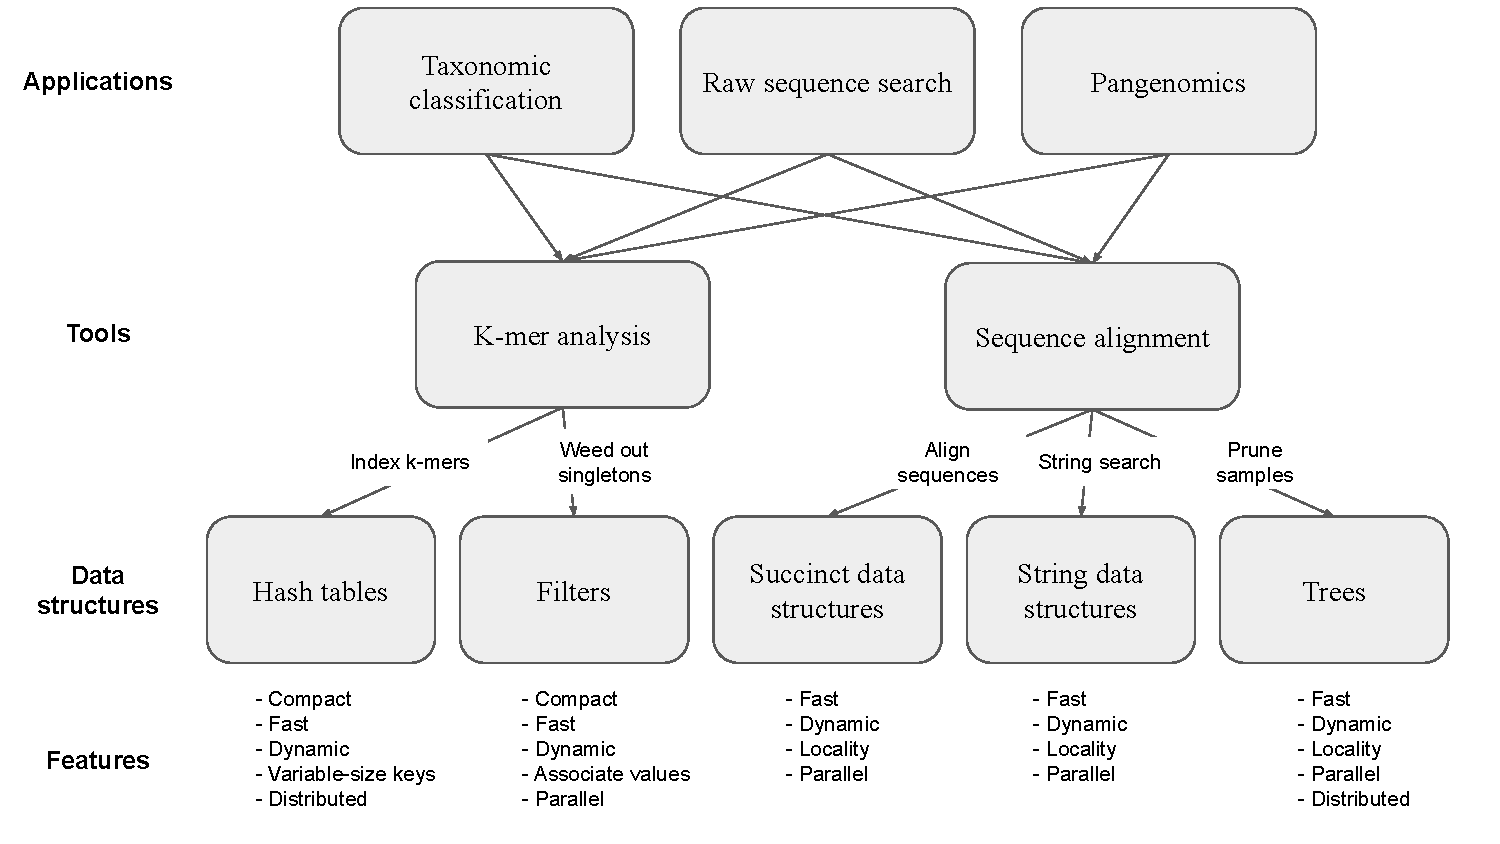
\includegraphics[width=0.75\textwidth]{images/PPOSS_App_DS}
\caption{Relation between computational-biology applications, data processing tools and data structures. We further mention the desired features in data structures to achieve performance and scalability.}
\label{fig1}
% \end{figure}
\end{wrapfigure}


\paragraph{Existing software tools for computational-biology applications.}

There are numerous tools for \kmer counting~\cite{MarccaisKi11,PandeyBJP17a}, sequence alignment~\cite{altschul1990basic,kielbasa2011adaptive,li2018minimap2,schwartz2003human}, raw sequence search~\cite{solomon2016fast,PandeyABFJP18Cell}, taxonomic classification~\cite{wood2014kraken,wood2019improved}, and pangenomics~\cite{garrison2018variation,pandey2021variantstore}. These tools rely on space-efficient and high-performance CPU data structures such as filters, sketches, hash tables, and string indexes. Most of these tools are designed for shared-memory parallelism and they often do not scale out of shared memory to disks.
These existing tools are limited by the single-node compute and shared-memory parallelism. They are not designed to scale to thousands of core on modern accelerators and scale out to hundreds to nodes in a high-performance computing (HPC) environment.
%
\prashant{I don't like the above paragraph much...}

% \begin{wrapfigure}{r}{0.4\textwidth}
% \centering
% 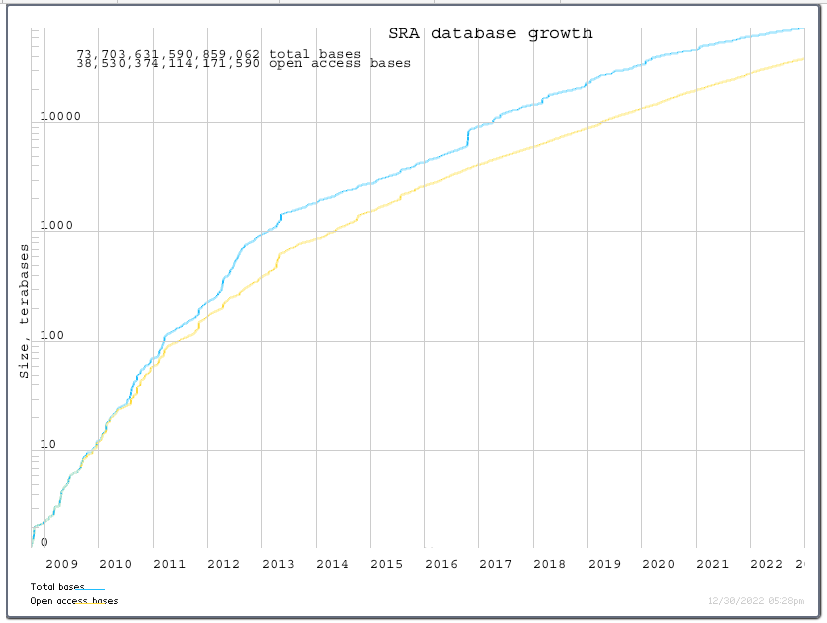
\includegraphics[width=0.95\textwidth]{images/SRA_data_growth.png}
% \caption{Sequence read archive (SRA) data growth. SRA data contains a trove of biological diversity information. Existing computational-biology tools do not scale to support searching through all of SRA. This renders what is otherwise an immensely valuable public resource largely inert.}
% \label{fig:sra_data}
% \end{wrapfigure}

\label{sec:we-need-performance-and-scalability}
\paragraph{CPU speed and RAM capacity cannot keep up with data growth.}
Unfortunately, CPU speed and RAM sizes aren't keeping up with the data growth in computational biology and other applications.
Although CPUs are increasing at 2--25\%/year and single-node RAM sizes are increasing at 2-11\%/year, genomics data is is likely to double in size every $1.5$ years~\cite{kodama2012sequence}.
Thus, today's software tools will not scale with tomorrow's data. For example, performing \kmer analysis or sequence alignment on petabyte-scale raw sequencing data is not possible on single-node shared-memory systems.

As mentioned by Leiserson et al.~\cite{leiserson2020there}, in the post Moore’s law period the performance gains will come from software, algorithms, and hardware (referred as the top of the computing stack) rather than the semiconductor (referred as the bottom). We can achieve massive scalability by, first designing data structures and algorithms to scale up using modern accelerators such as GPUs and second scaling out by using distributed memory in an high-performance computing (HPC) environment.


\paragraph{GPUs and other accelerators in computational biology.}
As with other high-performance computing (HPC) domains,
GPUs are increasingly used in large-scale computational biology because they offer orders of magnitude of jump in terms of low-cost parallelism, as long as data structure and algorithms can be defined to conform to the memory and parallelism requirement of GPUs.
%
For example, GPUs are used in some computational-biology applications to speed up \kmer counting~\cite{nisa2021distributed} and local assembly~\cite{awan2021accelerating}.
\prashant{Check if there are more examples.}

However, the penetration of GPUs into biology pipelines is limited by how the limitations of GPUs have translated so far into data structures.  These GPU limitations include:
\begin{enumerate}[noitemsep,nolistsep]
  \item GPU device RAM is much smaller than CPU RAM; this is especially
    challenging given the data sizes in computational biology.
  \item GPUs have high contention due to thousands of threads and are
    inefficient when computations are irregular.
  \item GPUs don't have a memory system; it is hard to perform dynamic memory management without involving the host CPU.
\end{enumerate}

These limitations affect the capabilities of GPU data structures: most existing GPU data structures do not support dynamic resizes and are statically allocated; pointer-based data structures such as trees and tries do not achieve high performance on GPUs; data structures on hard-to-align data, such as string or vectors, which have variable lengths are not available; data structures do not scale out of GPU device RAM to host.

These limitations are critical for building scalable computational-biology applications. For example, in \kmer analysis during raw sequence search and taxonomic classification the size of the \kmer multiset is not known in advance. Therefore, applications initialize the data structures such filters and hash tables to a default size and then dynamically resize (mostly expand) based on the actual number of \kmers. The ability to resize is critical to perform \kmer analysis in a space-efficient manner. Static data structures such as the hash tables and filters~\cite{GeilFO18} currently available on GPUs are sized using an over approximation of the number of \kmers which leads to space inefficiency.
Similarly, the local assembly module involves constructing thousands of hash tables in parallel and then using those hash tables to perform contig (contiguous strand of DNA) extension walks. The CPU implementation of local assembly relies heavily on dynamic
structures like hash tables, vectors and strings, which are a challenge to implement on GPUs. In addition, the algorithmic motif of local assembly induces a random memory-access pattern with a non-deterministic amount of work, which makes implementing this module on GPUs a very challenging problem.



% GPUs have not seen widespread adoption in computational biology applications. For example, they are used in taxonomic classification of metagenomic data, indexing and searching through terabytes of raw sequencing data, constructing and querying pangenomic graphs.

%Anything that involves sophisticated data structures and when memory is constrained GPUs are not currently useful.

% GPUs are not currently used for many computational biology applications because efficient GPU data structures do not exist.

\paragraph{Requirements for building scalable computational-biology applications}

Data structures are the core of computational-biology applications and are critical for their performance and scalability.
To build scalable computational-biology applications that can keep up with the rapid growth data we need compact, high-performance, dynamic, and distributed data structures. Specifically, we need: approximate data structures such as filters, sketches, and locality-sensitive hashing data structures; exact data structures such as hash tables, string data structures, succinct data structures, and trees.

These data structures and algorithms will need to exploit accelerators such as GPUs to scale up computations and at the same time support  features like space-efficiency, dynamism, high concurrency, scaling out of GPU device RAM to host RAM, and distributed memory design to scale out to multiple nodes.
%
Furthermore, to achieve fine-grained resizing and to keep the peak memory usage low we first need to develop new algorithmic approaches for traditional CPU data structures and then extend them to GPUs.

\subsection{Our proposed work}

We believe the answer to these challenges is a standalone library of memory-efficient, high-performance, dynamic, and scalable GPU data structures that can be directly used by computational biology applications that addresses the needs of emerging applications, allowing them to solve the problems described above.

\paragraph{Our approach is four-pronged.}  We will develop new \textbf{algorithmic theory} to design scalable data structures; we will develop new \textbf{systems} that implement our solutions in a scale-up manner,  both on CPU and GPU; we will a new framework to distribute our solutions in an \textbf{HPC} environment, so they  scale out to clusters of GPUs; and finally we will validate out solutions on \textbf{computational biology} workloads.
%
Specifically, out data structures are: \textbf{filters}, \textbf{hash tables}, \textbf{string indexes}, \textbf{sketches}, and related auxialiary data structures.  We will validate our solutions on \textbf{large-scale raw sequence search}, \textbf{taxonomic classification for metagenomic data}, \textbf{pangenomic indexing and analysis}, and others.

If successful we will be able to perform complex data analyses to answer biological questions on terabyte and petabyte scale datasets available. For example, raw sequencing data from SRA~\cite{kodama2012sequence}, metagenomic data from WA and Rhizo~\cite{hofmeyr2020terabase}, and pangenomic data from 100K genome project~\cite{XXX}. Existing data structures and software tools fail to scale to the data sizes making a these publicly-available and highly-valuable data resources largely inert.


The project’s novelties are: a vertical-stack approach spanning theory and algorithms: highly-concurrent, dynamic, and distributed data structures, systems: scale up using GPU acceleration, high-performance computing: scale out using distributed data structures, and applications: computational biology applications; new parallel and distributed data structures and algorithms to exploit the massive compute on GPUs applicable to other application domains; an API for developers to quickly and seamlessly integrate high-performance and scalable data structures in applications.
%
Our team includes a highly interdisciplinary team of researchers across four focus areas: applications (computational biology), theory and algorithms, systems, and high-performance computing. The team is taking a holistic theory/systems/HPC/applications co-design approach to explore four tightly interconnected research modules. These research modules are structured from bottom-up across the computing stack.


% \paragraph{Roadmap.} Roadmap here. In Section

% Section 2: bioinformatics problems, state of the art, what we need

% Section 3: Our approach: Why GPUs?  Also GPU-specific generic research problems

% Section 4: Filters, with reserach problems -- theory, systems, HPC

% Section 5: Hash tables, with reserach problems -- theory, systems, HPC

% Section 6: String indexes, with reserach problems -- theory, systems, HPC

% Section 7: Sketches, with reserach problems -- theory, systems, HPC

% Section 8: Bioinformatics validation, with research problems for each bioinformatics problem, and if successful statements.

\iffalse
==========



\begin{itemize}[noitemsep, leftmargin=*]
  \item {\bf Module 1 [theory/algorithms]:} Develop single-node GPU data structures.
    Specifically, filters, hash tables, succinct/string data structures, and
    trees. Challenges: high concurrency; being able to scale 100K threads;
    branching statements have a high cost; data movement and irregular data
    accesses are expensive. We will develop new theoretical data structures and
    algorithms that can efficiently exploit massive GPU parallelism while being
    compact and dynamic.

  \item {\bf Module 2 [Systems]:} Develop GPU data structures that can scale out of
      GPU device RAM to CPU host RAM. We will develop a memory allocator to
      seamlessly manage the GPU and CPU ram and efficiently move data across GPU
      and CPU RAMs.

    \item {\bf Module 3 [HPC]:} Develop data structures that can scale out to
      multiple-GPU nodes in a distributed computing environment. We will develop
      communication-efficient distributed versions of the above data structure
      to efficiently scale out hundreds of nodes in a HPC environment.

    \item {\bf Module 4 [Applications]:} Building high-performance and scalable
      computational biology applications by integrating GPU data structures in
      k-mer analysis, taxonomic classification, pangenomics tools.

\end{itemize}

-------------------------------------------------------------

In this project, we propose to develop a  collection of
memory-efficient, high-performance, dynamic, and distributed GPU data structures.
We will show how to use these data structures for our target applications in computational biology, as well as some others.
With the help these data structures, we aim to scale computational biology applications to massive datasets (raw sequencing datasets, metagenomic datasets from complex microbiomes, population-scale pangenomic datasets) and enable them to answer complex biological questions that are not possible today.
Because many of these applications require the same set of data structures, we will incorporate these data structures into a standalone library to enable easy reuse in other applications.

The PIs and others have shown that recent data structure advances~\cite{cite-somethin} show that
implementations that go beyond primitive data structures are possible on GPUs
but this work has not had much practical impact to date. \mfc{this is a big turd in teh middle of our first page -- well maybe the end of the first page -- is it even true? My papers with John are wracking up citatoins}    \mfc{awkward transition.  this is not about what we are proposing.  this comes before what we are proposing $\rightarrow$} A pure GPU solution is
desirable because transfer costs are high, and this is the direction being taken
in other application domains (machine learning, data science).

\paragraph{GPUs and other accelerators.}

In this project we envision solving these problems with a combination of  scale-up (via better algorithms and accelerators) and scale-out (distributing data and compute across multiple nodes of large high-performance computing systems). \mfc{how do you scale out without better algorithms?  you make it sounds like scaleup needs algorithms but any old crap will work for scaleout.  I don't think taht's true.}

% The rate of growth data is much higher than the growth of the CPU speeds and single-node storage capacities. CPU growth will not keep up with application demands.

Most existing applications in computational biology use CPUs to perform data  analysis.
However, the growth of the CPU speed and capacity is slowing and at the same time data is growing faster than ever. CPU growth will not keep up with application demands.

As a consequence, a few recent tools~\cite{cite-something} have tried to scale
up using accelerators like GPUs to speed up computations. However, these tools
use only primitive data structures and as a result achieve suboptimal
performance. Some applications [cite] have also tried to scale out using
distributed memory.  However, these applications are still limited by the CPU
speed and capacity and leave performance on the table due to suboptimal
scalability of data structures.


\prashant{Assigned to Martin/Michael: Need to add theory/algorithmic challenges
to develop GPU data structures. Why is it hard to just port existing CPU data
structures to GPUs.}


\begin{enumerate}[noitemsep, leftmargin=*]
  \item Filters
  \item Hash table
  \item String data structures (suffix array, FM index, BWT)
  \item Succinct data structures (Dynamic rank-select indexes)
  \item Trees and Tries
\end{enumerate}

\prashant{Martin, Michael wants a postdoc in year 3-4-5. Maybe a PhD student from John/Prashant.}


\prashant{Section 2: State of the art, data structures (theory/systems), applications. What are the deficiencies.}\\
\prashant{Section 3: Here's what we will do. Need a concrete plan with what we are going to. Sub-problems, milestones, schedule. How the four pillars interact.}\\
\prashant{Conclusion, Broader impact, previous NSF support}


%%%%%%%%%%%%%%%%%%%%%%%%%%%%%%
% Section 4: Management Plan %
%%%%%%%%%%%%%%%%%%%%%%%%%%%%%%
\section{Time Line and Management Plan}

\begin{table}[H]
\label{table1}
\renewcommand{\arraystretch}{0}
\caption{Project schedule.  PIs are Person One (P1), Person Two (P2), graduate student is GS, and the undergraduate student is US\@. Time frame gives the year each activity will occur.}
\scriptsize
\begin{tabularx}{\textwidth}{Y c c }
\hline
\hline
\textbf{Research Activity} & \textbf{Personnel} & \textbf{Time Frame}\\
\hline
Perform a task that sounds impressive & P2, US & Y1 \T\\
Perform another super-amazing task & P1, US & Y1 \T\\
Perform something else that may not be as sexy as the other things & P2, GS & Y1 \T\\
Wonder why you are such a terrible programmer & P1, US & Y1 \T\\
Analyze the results and stuff & P1, P2, SS & Y1,Y2 \T\\
Take the day off and grill some meat & P1, P2, SS & Y1,Y2 \T\\
Present findings at scientific meetings and publish results in peer-reviewed journals & P1, P2, US, GS & Y1, Y2, Y3\T\B\\
\hline
\hline
\end{tabularx}
\end{table}

\fi
